%%%%%%%%%%%%%%%%%%%%%%%%%%%%%%%%%%%%%%%%%%%%%%%%%%%%%%%%%%%%%%%%%%
%% Scribe Editors: 
%%    - Jimmy Lin <jimmy@utexas.edu>
%%    - Vutha Va <vutha.va@utexas.edu>
%%    - David Inouye <davidinouye@gmail.com>
%%%%%%%%%%%%%%%%%%%%%%%%%%%%%%%%%%%%%%%%%%%%%%%%%%%%%%%%%%%%%%%%%%
%% The main content of LECTURE 07 contains THREE SECTIONS. 
%% Specifically,
%%    ONE: definition and interpretations of Newton Method
%%    TWO: Affine Invariance of Newton Method
%%    THREE: Convergence Analysis of Newton Method
%%%%%%%%%%%%%%%%%%%%%%%%%%%%%%%%%%%%%%%%%%%%%%%%%%%%%%%%%%%%%%%%%%
%% Copyright (c), JIMMY, VUTHA, DAVID @ UT AUSTIN 2014
%%%%%%%%%%%%%%%%%%%%%%%%%%%%%%%%%%%%%%%%%%%%%%%%%%%%%%%%%%%%%%%%%%
\documentclass{beamer}
\mode<presentation>
\usepackage[latin1]{inputenc}
\usepackage{hyperref}
\usepackage{colortbl}
\usepackage{algorithmic}
\usepackage{times}
\usepackage{amssymb}
\usepackage{amsmath}
\usepackage{epsfig}

\usetheme{juanlespins}
\usepackage{graphicx}
\usepackage{bbm}

\setbeamertemplate{caption}[numbered]
\setbeamertemplate{navigation symbols}{} 
\title[Large Scale Optimization, Sanghavi, UT Austin]{EE 381V Large Scale Optimization: Lecture 07}
\author[Sanghavi]{Prof. Sujay Sanghavi}
\institute{The University of Texas at Austin\\ Scribes: Jimmy Lin, Vutha Va and David Inouye}
\date{\today}

\newcommand{\tr}{\text{Tr}}
\newcommand{\be}{\begin{eqnarray}}
\newcommand{\ee}{\end{eqnarray}}
\newcommand{\n}{\nonumber}
%\newcommand{\qed}{\hfill \blacksquare}

\renewcommand{\textfraction}{0}
%\renewtheorem{theorem}{Theorem}
%\newtheorem{lemma}{Lemma}
%\newtheorem{definition}{Definition}
\newtheorem{remark}{Remark}
\newtheorem{assumption}{Assumption}
\DeclareMathOperator{\dom}{dom}

\begin{document}

%%%%%%%%%%%%%%%%%%%%%%%%%%%%%%%%%%%%%%%%%%%%%%%%%%%%%%%%%%%%
%% TITLE PAGE
%%%%%%%%%%%%%%%%%%%%%%%%%%%%%%%%%%%%%%%%%%%%%%%%%%%%%%%%%%%%
\begin{frame}
\titlepage
\end{frame}

%%%%%%%%%%%%%%%%%%%%%%%%%%%%%%%%%%%%%%%%%%%%%%%%%%%%%%%%%%%%
%% Section ONE: definition and interpretations of Newton Method
%%%%%%%%%%%%%%%%%%%%%%%%%%%%%%%%%%%%%%%%%%%%%%%%%%%%%%%%%%%%
\newcommand{\fgrad}{\ensuremath{\nabla f(x)}}
\newcommand{\fhess}{\ensuremath{\nabla^2 f(x)}}
\newcommand{\fhessinv}{\ensuremath{\nabla^2 f(x)^{-1}}}
\newcommand{\xp}{\ensuremath{x^{+}}}
\newcommand{\dx}{\ensuremath{\Delta x}}
\begin{frame}
\frametitle{Newton Step}
\begin{definition}
    For $x \in \dom f,$ the vector 
    \be
    \dx_{nt} = - \fhessinv \fgrad
    \ee
    is called {\it Newton step} for function $f(\cdot)$, at point $x$. 
\end{definition}
In terms of positive definiteness of $\fhess$, 
\be
    \fgrad^T \dx_{nt} = -\fgrad^T \fhessinv \fgrad < 0
\ee
unless $\fgrad = 0$. So the Newton step is a descent direction unless $x$ is
already optimal.
\end{frame}

\begin{frame}
\frametitle{Interpretation I}
\framesubtitle{Minimizer of second-order Approximation}
    Second-order Taylor approximation $\hat{f}$ of $f$ at $x$ is
    \be
    \hat{f}(x+v) = f(x) + \fgrad^T v + \frac{1}{2} v^T \fhess v
    \ee
    where RHS is minimized at direction
    \be
        v = - \fhessinv \fgrad = \dx_{nt} 
    \ee
Combined with update rule, we have Newton update
    \be 
    \xp = x - t \fhessinv \fgrad
    \ee
    where $t$ is fixed step size.
\end{frame}

\begin{frame}
\frametitle{Interpretation I}
\framesubtitle{Minimizer of second-order Approximation}
\begin{figure}
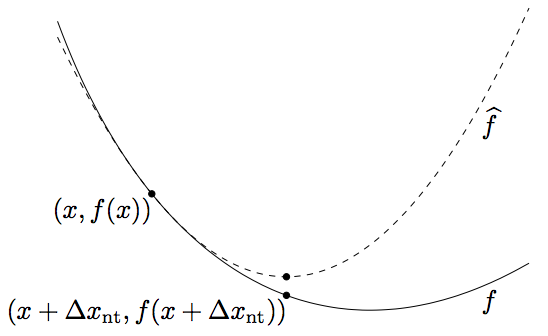
\includegraphics[width=2.2in]{figure/minimizer.png}
\caption{
The function $f$ (shown solid) and its second-order approximation
$\hat{f}$ at $x$ (dashed). The Newton step $\dx_{nt}$ is what must be added to $x$ to
give the minimizer of $\hat{f}$.
}
\label{fig:1}
\end{figure}
\end{frame}

\begin{frame}
\frametitle{Interpretation II}
\framesubtitle{Steepest descent direction in Hessian norm}
    Newton step can be interpreted as 
    steepest descent method when the norm is defined as
    \be
    \| u \|_{\fhess} \triangleq \sqrt{u^T \fhess u}
    \ee
    %%% TODO: add more comment
\end{frame}

\begin{frame}
\frametitle{Interpretation II}
\framesubtitle{Steepest descent direction in Hessian norm}
\begin{figure}
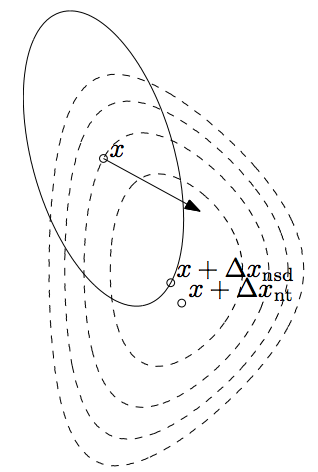
\includegraphics[width=1.3in]{figure/steepest.png}
\caption{
The dashed lines are level curves of a convex function. The ellipsoid shown
(with solid line) is $\{x + v | v^T \fhess v \leq 1\}$. The arrow shows
$-\fgrad$, the gradient descent direction. The Newton step $\dx_{nt}$ is the
steepest descent direction in the norm $\|\cdot \|_{\fhess}$.
}
\label{fig:2}
\end{figure}
\end{frame}

\begin{frame}
\frametitle{Interpretation III}
\framesubtitle{Solution of linearized optimality condition}
    Newton step can also be interpreted as 
    to linear approximation over gradient $\fgrad$ around $x$.
    \be
        \nabla f(x+v) \approxeq \fgrad + \fhess v
    \ee
    Set RHS to zero gives newton update.
    %%% TODO: add more comment
\end{frame}

\begin{frame}
\frametitle{Interpretation III}
\framesubtitle{Solution of linearized optimality condition}
\begin{figure}
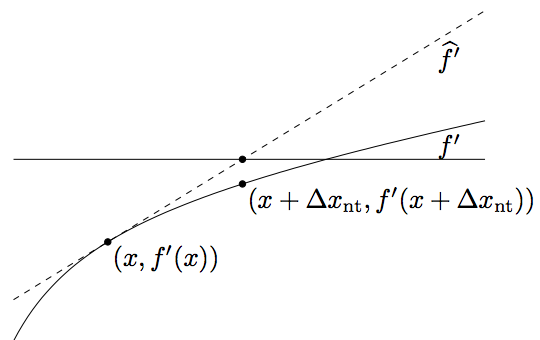
\includegraphics[width=2.5in]{figure/linear.png}
\label{fig:3}
\caption{
The solid curve is the derivative $f'$ of the function $f$ shown in Figure
\ref{fig:2}.
$\hat{f'}$ is the linear approximation of $f'$ at $x$. The Newton step
$\dx_{nt}$ is the difference between the root of $\hat{f'}$ and the point $x$.
}
\end{figure}
\end{frame}

%TODO: put first-order approximation a single slide? 
% with additional analysis maybe
%\begin{frame}
%\frametitle{Another Interpretation II}
%
%\end{frame}

%%%%%%%%%%%%%%%%%%%%%%%%%%%%%%%%%%%%%%%%%%%%%%%%%%%%%%%%%%%%
%% Section TWO: Affine Invariance of Newton step
%%%%%%%%%%%%%%%%%%%%%%%%%%%%%%%%%%%%%%%%%%%%%%%%%%%%%%%%%%%%
\newcommand{\yp}{\ensuremath{y^{+}}}
\newcommand{\gradient}[3]{\ensuremath{\nabla_{#1} #2 (#3)}}
\newcommand{\hessian}[3]{\ensuremath{\nabla^2_{#1} #2 (#3)}}
\newcommand{\inv}{^{-1}}
\begin{frame}
\frametitle{Affine Invariance of Newton step}
\begin{lemma}
    Newton step is affine invariant. 
\end{lemma}

For example, let $g(y) = f(Ay)$, $\yp$ be newton update on function
$g(\cdot)$, and 
$\xp$ be newton update on function $f(\cdot)$. 
Then if $x=Ay$, we have $\xp = A\yp$.

\begin{remark}
    Affine Invariance indicates that Newton Method is NOT vulnerable to the
    selection of coordinate system. 
\end{remark}
\begin{remark}
    Gradient Descent Method is not affine invariant. This means
    that bad coordinate choice may limit the power of Gradient Descent Method.
\end{remark}
\end{frame}

\begin{frame}
\frametitle{Proof of Affine Invariance}
    Let $x = Ay$ and $g(y) = f(Ay)$, then we have
    \be
    \hessian{y}{g}{y} &= \hessian{y}{f}{Ay} &= A^T \hessian{x}{f}{x} A \\
    \gradient{y}{g}{y} &= \gradient{y}{f}{Ay} &= A^T \gradient{x}{f}{x}
    \ee
    Newton update $\yp$ for $g(\cdot)$ can be extended as
    \be
    \yp &=& y - t(\hessian{y}{g}{y})\inv \gradient{y}{g}{y} \\
    &=& y - t(A^T \hessian{x}{f}{x} A)\inv A^T \gradient{x}{f}{x} \\
    &=& y - t\ A\inv \hessian{x}{f}{x}\inv \gradient{x}{f}{x}
    \ee
    Multiply both sides with affine tranformation $A$, 
    \be
    A\yp &=& Ay - A \cdot t\ A\inv \hessian{x}{f}{x}\inv \gradient{x}{f}{x} \\
    &=& x - t\ \hessian{x}{f}{x}\inv \gradient{x}{f}{x} \\
    &=& \xp
    \ee
\end{frame}
%%%%%%%%%%%%%%%%%%%%%%%%%%%%%%%%%%%%%%%%%%%%%%%%%%%%%%%%%%%%
%% Section three: Newton Method
%%%%%%%%%%%%%%%%%%%%%%%%%%%%%%%%%%%%%%%%%%%%%%%%%%%%%%%%%%%%

%%%%%%%%%%%%%%%%%%%%%%%%%%%%%%%%%%%%%%%%%%%%%%%%%%%%%%%%%%%%
%% Section Four: Convergence Analysis of Newton Method
%%%%%%%%%%%%%%%%%%%%%%%%%%%%%%%%%%%%%%%%%%%%%%%%%%%%%%%%%%%%
\begin{frame}
    \frametitle{Convergence Analysis: Assumption}    
    \begin{assumption}
        Let $f(\cdot)$ be the function discussed for Convergence of Newton
        Method. Both of following assumptions are what convergence analysis is
        based on.
        \begin{itemize}
            \item Function $f(\cdot)$ is strongly convex, such that
        \be
        m I \preceq \fhess \preceq M I
        \ee
    \item $\fhess$ is $L$-Lipschitz with constant $L > 0$, such that
        \be
        \| \hessian{}{f}{y} - \hessian{}{f}{x} \|_2 \leq L \|x-y\|_2,\ 
        \forall x,\ y
        \ee
        Note that induced matrix norm $\| \cdot \|_2$ equals to the largest
        singluar value of inside matrix.
        \end{itemize}
    \end{assumption}
\end{frame}

%% theorem for each phase and implication by each phase
\begin{frame}
    \frametitle{Convergence Analysis: Theorem}    
    \begin{theorem}[Part I]
        There exists $f,\ \eta,\ \gamma$, where $ 0 \leq \eta \leq \frac{m^2}{L}$,
        $\gamma = \frac{\alpha \beta m}{M^2}\eta^2$
        such that Newton Method with BTLS has two phases: 
        \begin{itemize}
            \item[(a)] Global or Damped Phase: If $\|\fgrad\|_2 \geq \eta$, then 
                \be
                f(\xp) - f(x) \leq -\gamma, \text{ also } 
                f(\xp) - f^* \leq c(f(x)-f^*) \label{CA:Theorem:phaseA}
                \ee
        \end{itemize}
    \end{theorem}
        Inequality \eqref{CA:Theorem:phaseA} has three implications: 
        \begin{itemize}
            \item Every newton step with BTLS gets closer to global optima by
                at least $\gamma$.
            \item Damped phase has at most $\frac{f(x^{(0)}) -
                    f^{*}}{\gamma}$ iterations.
            \item The damped phase essentially conforms to property of linear convergence.
        \end{itemize}
\end{frame}

\begin{frame}
    \frametitle{Convergence Analysis: Theorem}    
    \begin{theorem}[Part II]
        \begin{itemize}
            \item[(b)] Local or Quadratic Phase: If $\|\fgrad\|_2 < \eta$,
                then BTLS will give $t = 1$ and we have
                \be
                \frac{L}{2m^2} \|\gradient{}{f}{\xp}\|_2 \leq 
                    \bigg(\frac{L}{2m^2} \|\fgrad\|_2 \bigg)^2
                \ee
        \end{itemize}
    \end{theorem}
    Implications:
    \begin{itemize}
    \item To achieve an accuracy of $\epsilon$, only $O(\log \log \epsilon)$ iterations are needed once in the quadratic phase.
    \item Also, for strongly convex functions, $f(x) \to p*$ quadratically.
    \end{itemize}
\end{frame}

% TODO: proof of step size t = m/M satisfies the exit condition for BTLS
\begin{frame}
    \frametitle{Convergence Analysis: Proof Part (a)}    
    \begin{lemma}[BTLS Damped Lemma]
        $t = \frac{m}{M}$ satisfies the exit condition of BTLS.
    \end{lemma}
    Proof omitted because of space.  See p. 489-490 in Boyd.
    \begin{lemma}[Damped Phase]
        If $\|\fgrad\|_2 \geq \eta$, 
        then $f(\xp) - f(x) \leq -\gamma$, 
        where  $\gamma = \frac{\alpha \beta m}{M^2}\eta^2$
    \end{lemma}
\end{frame}

% TODO: proof of inequality for (a) phase and show linear convergence
% inequality
\begin{frame}
    \frametitle{Convergence Analysis: Lemma Damped Phase}    
	\begin{align}
	t &\leq \beta \frac{m}{M} \tag{BTLS Damped Lemma} \\
	f(x^+) &\leq f(x) - \alpha\left(\beta \frac{m}{M} \right) g^T H^{-1} g \tag{BTLS condition} \\
	&\leq f(x) - \alpha\left(\beta \frac{m}{M} \right) \left(\frac{1}{M}\|g\|_2^2 \right) \tag{$H^{-1} \preceq I/m$} \\
	&= f(x) - \alpha\beta \frac{m}{M^2}\|g\|_2^2 \notag \\
	&= f(x) - \underbrace{\alpha\beta \frac{m}{M^2} \eta^2}_{\gamma} \tag{Assumptions}
	\end{align}  
	\begin{align}
	\implies f(x^+) - f(x) = - \gamma
	\end{align}
\end{frame}

% TODO: proof of inequality for (b) phase
\begin{frame}
    \frametitle{Convergence Analysis: Proof Part (b)}
    \begin{lemma}[BTLS Quad. Lemma]
        With the assumptions in (b), $t = 1$ satisfies the exit condition of BTLS.
    \end{lemma}
    Proof omitted because of space.  See p. 490-491 in Boyd.
    \begin{lemma}[Quad. Phase]
        If $\|\fgrad\|_2 < \eta$, then 
        $ \frac{L}{2m^2} \|\gradient{}{f}{\xp}\|_2 \leq
                \bigg(\frac{L}{2m^2} \|\fgrad\|_2 \bigg)^2 $
    \end{lemma}

\end{frame}

\begin{frame}
    \frametitle{Convergence Analysis: Quad. Phase}
    \begin{align}
    x^+ &= x - H^{-1}g \tag{BTLS Quad. Lemma} \\
    \| \nabla f(x^{+})\|_2 &= \| \nabla f(x-H^{-1}g) - g + HH^{-1}g \|_2 \tag{Add zero} \\
	&= \left\|\int_{0}^{1} \nabla^2 f(x-tH^{-1}g) (-H^{-1}g) + HH^{-1}g \mathrm{d}t \right\|_2 \tag{Fund. Theorem of Calculus} \\
	&= \left\| \int_{0}^{1} (\nabla^2 f(x-tH^{-1}g) - H) (-H^{-1}g) \mathrm{d}t \right\|_2 \tag{Rearrange} \\
	&\leq \int_{0}^{1} \left\| (\nabla^2 f(x-tH^{-1}g) - H)\right\|_2 \left\| (-H^{-1}g)\right\|_2 \mathrm{d}t  \tag{Triangle inequality of norms}
    \end{align}
\end{frame}

\begin{frame}
    \frametitle{Convergence Analysis: Quad. Phase}
    \begin{align}
    \| \nabla f(x^{+})\|_2 &\leq \int_{0}^{1} \left\| (\nabla^2 f(x-tH^{-1}g) - H)\right\|_2 \|H^{-1}g\|_2 \mathrm{d}t \notag \\
	&\leq \int_{0}^{1} L \| \!\!-\!tH^{-1}g \|_2 \|H^{-1}g\|_2 \mathrm{d}t \tag{Liptschitz Continuity of Hessian} \\
	&= L \|H^{-1}g\|_2^2 \int_{0}^{1} t \mathrm{d}t = \frac{L}{2} \|H^{-1}g\|_2^2 \notag \\	
	&\leq \frac{L}{2m^2} \|g\|_2^2 \tag{Strong convexity ($H^{-1} \preceq I/m$)}
	\end{align}
	\begin{align}
 	\implies \frac{L}{2m^2} \| \nabla f(x^{+})\|_2 &\leq \left( \frac{L}{2m^2} \|g\|_2 \right)^2
    \end{align}
\end{frame}

%%%%%%%%%%%%%%%%%%%%%%%%%%%%%%%%%%%%%%%%%%%%%%%%%%%%%%%%
%%%%%%%%%%%%%%%%%%%%%%%%%%%%%%%%%%%%%%%%%%%%%%%%%%%%%
\end{document}
